\documentclass[11pt, a4paper]{article}

\usepackage[english]{babel}
\usepackage[utf8]{inputenc}
\usepackage[T1]{fontenc}
\usepackage{lmodern}
\usepackage[top=2.5cm, bottom=2.5cm, left=2.5cm, right=2.5cm]{geometry}
\usepackage{booktabs}
\usepackage{array}
\usepackage{xcolor}
\usepackage{graphicx}
\usepackage[hidelinks, colorlinks=true,
            linkcolor=blue!55!black,
            citecolor=green!40!black,
            urlcolor=blue!55!black]{hyperref}
\usepackage{amsmath}
\usepackage{amssymb}
\usepackage{microtype}
\usepackage{caption}
\usepackage{parskip}
\usepackage{tikz}
\usetikzlibrary{arrows.meta, positioning, shapes.geometric}
\usepackage{footmisc}

\title{\textbf{Il divario semantico tra priorit\`a giovanili\\
       e agenda comunicativa dei leader politici italiani}\\[0.4em]
       \large Un'analisi computazionale di Instagram a partire dal Flash
              Eurobarometro EP013EP}

\author{Marco Coppola \and Davide De Rosa \and Marco Miozza \and Valerio Pio De Nicola\\[0.3em]
  \small Alma Mater Studiorum --- Universit\`a di Bologna\\
  \small Corso di Human Data Science, A.A.\ 2025/2026}

\date{Maggio 2026}

\begin{document}
\maketitle

\begin{abstract}
\noindent
Il presente studio misura quanto l'agenda tematica dei leader politici
italiani su Instagram si avvicini a quella che i giovani italiani fra i 16
e i 30 anni dichiarano prioritaria nel Flash Eurobarometro
EP013EP~\cite{ep2024youth}, basato sui dati della domanda Q2 dell'edizione
2024 della survey. Tre profili coprono i tre principali partiti italiani
secondo le elezioni politiche del 2022~\cite{italianelections2022}, ovvero
Schlein per il PD, Meloni per FdI e Conte per il M5S. Per ognuno lo
scraping di Instagram raccoglie i post pubblicati fra settembre 2025 e
febbraio 2026 e per ciascun post la caption, l'OCR delle immagini e la
trascrizione audio dei reel vengono fusi in un'unica rappresentazione
testuale e classificati da un Large Language Model locale, che assegna un
punteggio Likert $1$--$5$ sui dieci temi rilevati dall'Eurobarometro.
L'unit\`a di confronto \`e il \textbf{Coverage Rate} di un tema, ovvero la
proporzione di post di un politico in cui il modello assegna a quel tema
un punteggio $\geq 3$, soglia che corrisponde a un tema chiaramente
riconoscibile. Il confronto avviene sui \textit{ranking} dei dieci temi e
non sui valori grezzi, dato che percentuali di selezione in una survey
\textit{pick top-3} e Coverage Rate prodotti da un'analisi testuale
automatica vivono su scale incommensurabili. Il modello
\texttt{gemma4:e4b} \`e stato validato contro la media di quattro
annotatori umani su un campione di $30$ post, ottenendo un $\kappa_w$ di
Cohen pari a $0{,}78$. L'analisi rivela un disallineamento ampio e
trasversale, dato che nessun politico raggiunge una correlazione di
Spearman con il ranking giovanile superiore a $0{,}19$ e il tema
\emph{ambiente e clima}, primo per i giovani, compare nel terzo inferiore
delle classifiche di tutti e tre i profili. Specularmente
\emph{democrazia e legalit\`a}, che fra i giovani occupa il rank
$8{,}5$, \`e il tema in testa alla classifica per tutti e tre i politici.
\end{abstract}

\section{Introduzione}

La distanza fra ci\`o di cui i giovani europei dicono di preoccuparsi e
ci\`o di cui i loro rappresentanti politici parlano in pubblico \`e uno
dei temi ricorrenti della letteratura recente sulla disaffezione politica
giovanile~\cite{ep2024youth, eurobarometer_program}. La domanda di
ricerca del presente studio \`e se nei contenuti che i principali leader
politici italiani pubblicano su Instagram l'ordine di priorit\`a dei
dieci temi rilevati dall'Eurobarometro 2024 sia compatibile con l'ordine
dichiarato dai giovani italiani. L'impostazione si rif\`a al filone
classico dell'\textit{agenda-setting}~\cite{mccombs1972}, in cui la
salienza di un tema nel discorso pubblico viene operativizzata come la
frequenza con cui quel tema viene scelto per essere comunicato. Su
Instagram questa frequenza pu\`o essere stimata in modo sistematico a
partire da un campione esaustivo dei post di un profilo.

Per ogni profilo le due classifiche dei dieci temi, una stimata sui
giovani e l'altra sui post Instagram, sono confrontate sia globalmente,
tramite Spearman $\rho$ e Kendall $\tau_b$, sia localmente, tramite il
\textit{rank gap} per singolo tema e l'indice Top-$K$ Jaccard sui temi
pi\`u salienti. Con $n=10$ temi, dimensione fissata dal protocollo
dell'Eurobarometro, le correlazioni globali sono riportate come misure
descrittive della distanza fra le due classifiche, mentre l'analisi
pi\`u informativa avviene per singolo tema.

Vengono analizzati i profili Instagram dei leader dei tre principali
partiti italiani secondo le elezioni politiche del
2022~\cite{italianelections2022}, ovvero Giorgia Meloni per FdI con
account \texttt{giorgiameloni}, Elly Schlein per il PD con account
\texttt{ellyesse} e Giuseppe Conte per il M5S con account
\texttt{giuseppeconte\_ufficiale}. I tre profili hanno un'attivit\`a
Instagram comparabile per volume di post nel periodo considerato e
costituiscono il sotto-insieme statisticamente robusto del campione
iniziale.

\section{Sorgenti dei dati}

\subsection{Flash Eurobarometro EP013EP}

Il Flash Eurobarometro EP013EP, parte del programma Eurobarometro del
Parlamento Europeo~\cite{eurobarometer_program}, \`e una survey
commissionata dalla Direzione Generale per la Comunicazione e
somministrata in tutti i 27 Stati membri fra l'agosto e l'ottobre 2024,
con campione complessivo intorno a $26\,000$ rispondenti fra i 16 e i 30
anni~\cite{ep2024youth}. La sezione italiana \`e stata raccolta nel mese
di settembre--ottobre 2024 con campionamento stratificato per et\`a,
genere e area geografica, secondo la metodologia ufficiale documentata
nei \textit{Technical Specifications}
dell'indagine~\cite{ep2024youth_methodology}. L'edizione 2024 della
survey viene presa in questo studio come unica rilevazione affidabile e
direttamente utilizzabile della distribuzione delle priorit\`a giovanili
italiane su uno spettro tematico ampio, dato che si tratta della
pubblicazione pi\`u recente del Parlamento Europeo dedicata a questo
target.

La domanda usata in questo studio \`e Q2, formulata come
\textit{``Among the following, which three issues should be tackled as a
priority by the European Union over the next five years?''}. Si tratta
di una domanda di tipo \textit{pick top-3}, in cui il rispondente
seleziona \emph{fino a tre} temi da una lista chiusa di dodici voci,
costituita dai dieci temi pi\`u due opzioni esclusive, \textit{Other} e
\textit{None of these / Don't know}. Le due opzioni esclusive sono
mutualmente incompatibili con le altre.

La variabile sottostante \`e binaria a livello di rispondente per
ciascun tema, dato che il tema risulta selezionato oppure non
selezionato. La percentuale riportata in Tabella~\ref{tab:youth} per il
tema $i$ \`e quindi la stima della proporzione $\Pr(\text{tema } i
\text{ scelto})$ nella popolazione giovanile italiana. La somma delle
dieci percentuali non raggiunge il limite teorico del $300\%$ per due
ragioni concorrenti. La prima \`e che le opzioni esclusive
\textit{Other} e \textit{None} sottraggono rispondenti dal denominatore
di tutte le altre. La seconda \`e che la formulazione del quesito
ammette la selezione \emph{fino a tre} temi e una porzione non
trascurabile dei rispondenti ne sceglie meno di tre. Sulla riga Italia
la somma osservata si colloca attorno al $257\%$, in linea con una media
di circa $2{,}57$ scelte per rispondente.

\begin{table}[!htbp]
\centering
\caption{Riga Italia di EP013EP Q2 con la percentuale di rispondenti che
hanno selezionato il tema fra le tre principali sfide UE. I rank tengono
conto dei pareggi tramite la convenzione del rank medio.}
\label{tab:youth}
\small
\begin{tabular}{r l r}
\toprule
\textbf{Rank} & \textbf{Tema} & \textbf{\%} \\
\midrule
 1.0 & Ambiente e clima         & 46 \\
 2.0 & Lavoro e economia        & 38 \\
 3.5 & Costo della vita         & 34 \\
 3.5 & Salute e welfare         & 34 \\
 5.0 & Istruzione e formazione  & 26 \\
 6.0 & Uguaglianza di genere    & 24 \\
 7.0 & Difesa e sicurezza       & 16 \\
 8.5 & Immigrazione             & 15 \\
 8.5 & Democrazia e legalit\`a  & 15 \\
10.0 & Abitazione               &  9 \\
\bottomrule
\end{tabular}
\end{table}

\subsection{Contenuti Instagram}

La scelta di Instagram come piattaforma di osservazione \`e supportata
dallo stesso Eurobarometro EP013EP~\cite{ep2024youth}, che indica nei
giovani italiani $16$--$30$ anni Instagram come primo canale digitale
per l'informazione politica. TikTok occupa una posizione comparabile,
ma formato e pubblico sono in larga parte sovrapposti, e nella prassi
osservata i contenuti pubblicati dai politici italiani su TikTok sono
per la quasi totalit\`a gli stessi reel pubblicati su Instagram tramite
cross-posting. Instagram \`e quindi il canale singolo che cattura la
maggior parte del segnale comunicativo rivolto al pubblico giovane
italiano.

I post analizzati coprono la finestra settembre 2025 -- febbraio 2026.
La scelta di questa finestra temporale \`e arbitraria e funge da blocco
di osservazione fissato in modo identico per i tre profili, in modo da
rendere i Coverage Rate confrontabili fra loro a parit\`a di periodo. I
risultati vanno letti come riferiti a quel preciso intervallo e ranking
diversi sono in linea di principio possibili su finestre alternative.

L'edizione EP013EP della survey \`e di settembre--ottobre 2024, mentre
la finestra di osservazione dei post \`e di settembre 2025 -- febbraio
2026. L'analisi accetta dunque uno scostamento temporale di circa un
anno fra le due fonti, dato che l'edizione 2024 dell'Eurobarometro \`e
la rilevazione UE pi\`u recente disponibile sulle priorit\`a giovanili
italiane su questo spettro tematico.

La numerosit\`a dei campioni varia per profilo, con
$N_{\text{Schlein}}=233$, $N_{\text{Meloni}}=278$ e
$N_{\text{Conte}}=231$. La variabilit\`a di $N$ riflette la differente
intensit\`a comunicativa dei tre leader nel periodo considerato. Le
metriche utilizzate sono tutte \textit{ratio}, ovvero Coverage Rate,
$\rho$, $\tau_b$ e Jaccard, e quindi confrontabili tra profili anche con
$N$ diversi, fermo restando che gli intervalli di confidenza sui
Coverage Rate sono pi\`u larghi sui profili meno attivi.

Lo scraping \`e effettuato tramite la libreria \textit{instaloader}
\cite{instaloader} con sessione autenticata. Vengono raccolti soltanto
i post pubblici, senza commenti, follower o metadati personali, in
linea con un'impostazione minimale rispetto al GDPR.

\section{Pipeline di elaborazione}

L'elaborazione \`e organizzata in cinque stadi sequenziali, illustrati
in Figura~\ref{fig:pipeline}. I dettagli implementativi, quali parser,
retry policy e gestione degli errori, sono documentati nel repository
del progetto e questa sezione si limita agli aspetti rilevanti per la
validazione della qualit\`a dei dati prodotti.

\begin{figure}[!htbp]
\centering
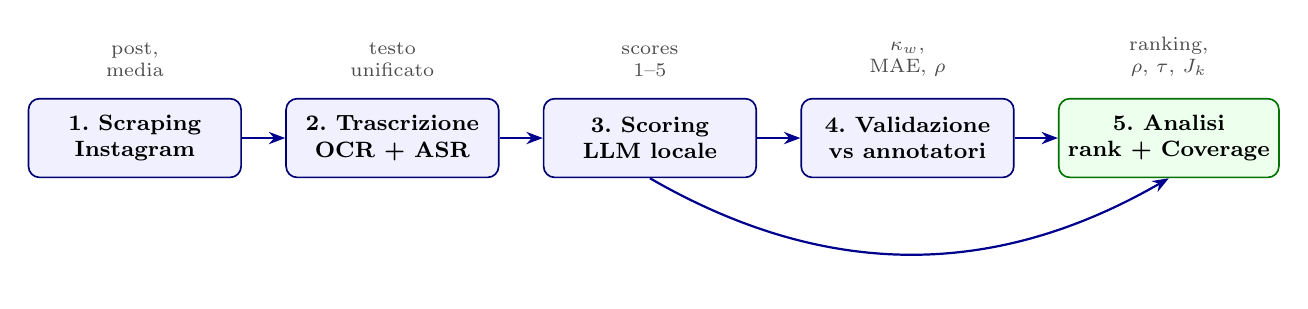
\begin{tikzpicture}[
  node distance=0.55cm,
  box/.style={draw=blue!45!black, rounded corners=4pt, fill=blue!6,
              minimum width=2.7cm, minimum height=1.0cm, align=center,
              font=\footnotesize\bfseries, line width=0.6pt},
  outb/.style={draw=green!45!black, rounded corners=4pt, fill=green!7,
              minimum width=2.7cm, minimum height=1.0cm, align=center,
              font=\footnotesize\bfseries, line width=0.6pt},
  arr/.style={-{Stealth[scale=0.9]}, thick, blue!55!black},
  lbl/.style={font=\scriptsize, gray!60!black, align=center}
]
\node[box]                       (s1) {1.\ Scraping\\Instagram};
\node[box, right=of s1]          (s2) {2.\ Trascrizione\\OCR + ASR};
\node[box, right=of s2]          (s3) {3.\ Scoring\\LLM locale};
\node[box, right=of s3]          (s4) {4.\ Validazione\\vs annotatori};
\node[outb, right=of s4]         (s5) {5.\ Analisi\\rank + Coverage};
\draw[arr] (s1) -- (s2);
\draw[arr] (s2) -- (s3);
\draw[arr] (s3) -- (s4);
\draw[arr] (s3.south) to[out=-30, in=-150] (s5.south);
\draw[arr] (s4) -- (s5);
\node[lbl, above=0.15cm of s1] {post,\\media};
\node[lbl, above=0.15cm of s2] {testo\\unificato};
\node[lbl, above=0.15cm of s3] {scores\\1--5};
\node[lbl, above=0.15cm of s4] {$\kappa_w$,\\MAE, $\rho$};
\node[lbl, above=0.15cm of s5] {ranking,\\$\rho$, $\tau$, $J_k$};
\end{tikzpicture}
\caption{Pipeline a cinque stadi in cui lo scoring LLM dello stadio 3
alimenta sia la validazione dello stadio 4 sia l'analisi finale dello
stadio 5.}
\label{fig:pipeline}
\end{figure}

I post Instagram veicolano testo nella caption, in overlay grafici sulle
immagini e nell'audio dei reel. Tutte le componenti vengono ridotte a
un'unica rappresentazione testuale tramite OCR sulle immagini con
Tesseract e trascrizione automatica con
\textit{faster-whisper}~\cite{fasterwhisper} nel modello
\texttt{large-v3-turbo}. La qualit\`a delle componenti automatiche \`e
quella standard delle pipeline open-source per l'italiano, con
trascrizione audio affidabile sul parlato chiaro e OCR affidabile su
slogan e infografiche pulite, ma peggiore su scritte stilizzate.
Eventuali errori a livello di singolo lessema sono assorbiti a valle
dallo scoring LLM, che lavora sull'evidenza tematica diffusa nel testo
e non su occorrenze puntuali di parole-chiave.

Ogni post viene poi classificato da un Large Language Model servito
localmente attraverso \textit{Ollama}~\cite{ollama}. Il prompt richiede
in un'\emph{unica} risposta JSON il punteggio Likert $1$--$5$ sui dieci
temi, calibrati gli uni rispetto agli altri. Il decoding \`e
deterministico, con \texttt{temperature}$=0$, per garantire la
riproducibilit\`a degli score su input fisso.

La rubrica utilizzata sia dall'LLM sia dagli annotatori umani \`e la
medesima ed \`e intenzionalmente asimmetrica, con un vero ``zero'' al
livello $1$. I cinque livelli vanno da tema completamente assente, a
tema appena accennato, a tema riconoscibile anche se secondario, a
tema significativo trattato con profondità, fino a tema oggetto
principale del post. La soglia di salienza usata in tutta l'analisi \`e
$\tau = 3$, ovvero un post viene considerato a copertura di un tema
quando il modello gli assegna un punteggio almeno pari a $3$. La
giustificazione di questa soglia \`e discussa in \S\ref{sec:coverage}.

\section{Validazione del modello}

\subsection{Disegno dell'esperimento}

Tre modelli open-weight sono stati confrontati come potenziali
annotatori automatici, ovvero Gemma~4 E4B~\cite{gemma2024}, LLaMA~3.1
8B-Instruct e Qwen3 14B. Ciascun modello ha annotato un campione di
validazione di $30$ post, dieci per profilo, sulla rubrica Likert
descritta nella sezione precedente. Gli stessi post sono stati annotati
indipendentemente da quattro annotatori umani, e la media arrotondata
per difetto delle loro annotazioni costituisce il riferimento contro
cui ogni modello \`e stato misurato. Si tratta dunque di $300$
osservazioni appaiate per modello.

\subsection{Metriche di accordo}

L'accordo modello-umano viene misurato lungo cinque dimensioni
complementari, ciascuna scelta per coprire un aspetto specifico
dell'errore. L'errore medio assoluto MAE quantifica lo scarto medio
modello-umano in punti scala e fornisce un'unit\`a immediatamente
interpretabile. Il $\kappa_w$ di Cohen con pesi quadratici misura
l'accordo inter-rater corretto per il caso, penalizzando in modo
quadratico le distanze fra i livelli, condizione particolarmente adatta
a una scala ordinale di soli cinque livelli, ed \`e interpretato
secondo la banda di Landis e Koch~\cite{landis1977}. La correlazione
di Spearman $\rho$ valuta l'accordo sull'ordinamento, indipendentemente
dal valore numerico assoluto delle annotazioni. L'$\alpha$ di
Krippendorff in variante ordinale fornisce una seconda stima della
reliability, robusta a categorie sbilanciate~\cite{krippendorff2004}.
Il bias medio degli scarti modello-umano completa il quadro.

Il test del $\chi^2$ \`e stato esplicitamente escluso. Il motivo
principale \`e che il $\chi^2$ tratta le cinque categorie della scala
come puramente nominali, ignorando l'ordinamento naturale che \`e
invece centrale in una scala Likert, cosicch\'e dal suo punto di vista
uno scarto $1\!\leftrightarrow\!5$ equivale a uno
$3\!\leftrightarrow\!4$. A questo si aggiunge che il $\chi^2$ classico
non sfrutta l'appaiamento osservazione-per-osservazione fra modello e
umani e che con tabelle di contingenza $5\times 5$ a soli $30$ post per
politico le frequenze attese in molte celle scendono al di sotto della
soglia di cinque, condizione che invalida l'approssimazione asintotica
della distribuzione $\chi^2$. Tutte e tre le ragioni suggeriscono di
preferire metriche pensate per dati ordinali appaiati, quali $\kappa_w$
e $\alpha$ ordinale.

\subsection{Risultati}

Il modello \texttt{gemma4:e4b} \`e adottato per lo scoring complessivo
dei $742$ post sulla base di tre criteri convergenti. Il primo \`e il
MAE pi\`u basso fra i tre, pari a $0{,}244$ contro lo $0{,}282$ di Qwen
e lo $0{,}473$ di LLaMA. Il secondo \`e un bias medio contenuto, pari a
$+0{,}10$ contro $+0{,}21$ e $+0{,}41$. Il terzo \`e la dimensione
inferiore del modello, $4$B contro i $14$B di Qwen, che riduce il
costo di inferenza su un dataset di centinaia di post. Il $\kappa_w$
risulta sostanzialmente equivalente a quello di Qwen, con valore
$0{,}784$ contro $0{,}780$, e non discrimina di per s\'e fra i due,
come riportato in Tabella~\ref{tab:val}.

\begin{table}[!htbp]
\centering
\caption{Validazione dei tre modelli LLM contro la media di quattro
annotatori umani su $30$ post, con la banda interpretativa di Landis e
Koch.}
\label{tab:val}
\small
\begin{tabular}{l r r l r r r}
\toprule
\textbf{Modello} & \textbf{MAE} & \textbf{$\kappa_w$} & \textbf{Livello} &
\textbf{Spearman $\rho$} & \textbf{Krippendorff $\alpha$} & \textbf{Bias} \\
\midrule
gemma4:e4b             & 0.244 & 0.784 & Buono     & 0.742 & 0.783 & $+0.10$ \\
qwen3:14b              & 0.282 & 0.780 & Buono     & 0.757 & 0.778 & $+0.21$ \\
llama3.1:8b-instruct   & 0.473 & 0.601 & Buono     & 0.728 & 0.588 & $+0.41$ \\
\bottomrule
\end{tabular}
\end{table}


\subsection{Overshooting per topic}

L'errore decomposto per tema, riportato in Figura~\ref{fig:bias},
mostra che il bias positivo del modello scelto si concentra in due
aree, ovvero \emph{democrazia e legalit\`a} con bias $+0{,}37$ e MAE
$0{,}58$ ed \emph{difesa e sicurezza} con bias $+0{,}05$ e MAE
$0{,}55$. Negli altri otto temi il bias \`e trascurabile, con un'unica
eccezione di segno opposto sull'immigrazione, che presenta un bias di
$-0{,}07$ il cui ordine di grandezza \`e tuttavia compatibile con il
rumore campionario di $30$ osservazioni e non costituisce un pattern
sistematico.

Per \textit{overshooting} si intende la tendenza del modello a
sovrastimare la rilevanza di un tema rispetto al riferimento umano. Non
si tratta di un errore casuale, che sarebbe altrimenti assorbito nel
MAE complessivo, bens\`{\i} di uno scostamento condizionale verso
l'alto della distribuzione delle annotazioni del modello. In presenza
di un post che tocca anche solo marginalmente uno dei due temi
sensibili, il modello tende a classificarlo a livello $3$ o $4$,
mentre gli annotatori umani sono pi\`u parsimoniosi e si fermano al
livello $2$. L'effetto \`e particolarmente forte sui temi a forte
cornice retorica generica, come richiami al patto sociale, allo Stato
di diritto o alla difesa nazionale. L'LLM riconosce i lessemi
caratteristici e attiva il tema, mentre gli umani contestualizzano e
interpretano la presenza dei lessemi come decorativa. Le conclusioni
dell'analisi sui due temi \emph{democrazia/legalit\`a} e
\emph{difesa/sicurezza} sono pertanto da leggere con cautela, dato che
una porzione del Coverage Rate osservato pu\`o essere attribuita al
bias del modello e non a una scelta editoriale dei politici.

\begin{figure}[!htbp]
\centering
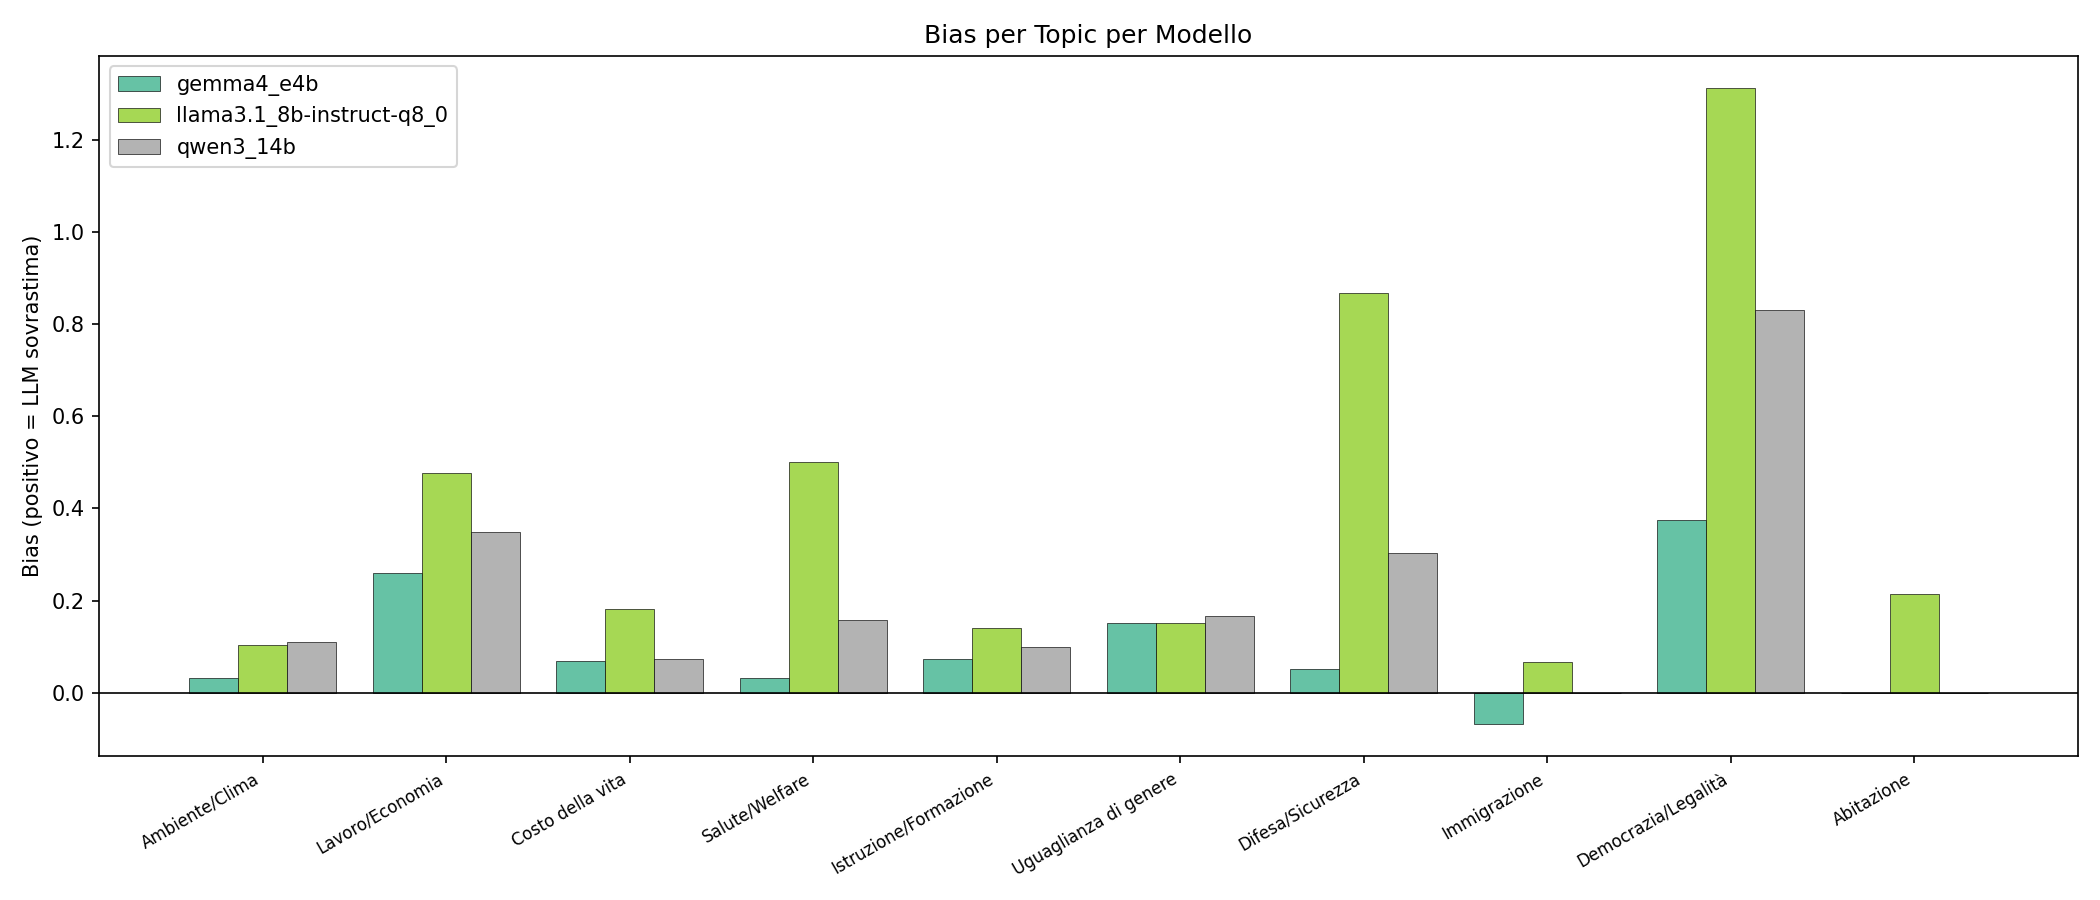
\includegraphics[width=0.95\textwidth]{bias_per_topic.png}
\caption{Bias del modello \texttt{gemma4:e4b} per topic. Valori
positivi indicano sovrastima rispetto agli annotatori umani e lo
scostamento si concentra su \emph{democrazia/legalit\`a}.}
\label{fig:bias}
\end{figure}

\subsection{Affidabilit\`a del riferimento umano}

La validazione misura l'accordo del modello con la media di quattro
annotatori umani, non con una verit\`a oggettiva. Gli annotatori umani
stessi non sono infallibili, dato che la classificazione tematica con
una rubrica Likert su un post breve e multimodale \`e un compito
interpretativo, e l'accordo fra umani su task analoghi in letteratura
si attesta tipicamente su $\kappa$ tra $0{,}5$ e
$0{,}8$~\cite{artstein2008}. Il riferimento costruito \`e dunque una
stima ragionevole, non un \textit{ground truth} in senso stretto. I
rank complessivi sono robusti al \emph{rumore casuale} per-post, dato
che errori di un punto scala su singoli post si compensano in media,
e la sensitivity analysis rispetto a $\tau$ presentata in
\S\ref{sec:coverage} mostra che l'ordinamento globale dei dieci temi
rimane stabile a perturbazioni del cutoff di salienza, ulteriore
indicazione che le conclusioni non sono guidate da fluttuazioni
locali della scala Likert.

\section{Metriche di allineamento}

\subsection{Coverage Rate per tema}\label{sec:coverage}

Per ciascun politico $p$ e tema $i$ definiamo il \textbf{Coverage
Rate} come
\[
  c_i^{(p)} \;=\; \frac{1}{N_p}\sum_{j=1}^{N_p}
  \mathbf{1}\!\left[s_{i,j}^{(p)} \geq \tau\right],
\]
con $s_{i,j}^{(p)}\in\{1,\dots,5\}$ il punteggio Likert sul tema $i$
nel post $j$, $N_p$ il numero di post del politico, e $\tau=3$ la
soglia di salienza coerente con la rubrica Likert descritta nella sezione precedente. La
funzione indicatrice $\mathbf{1}[\cdot]$ \`e definita come
\[
  \mathbf{1}[\text{condizione}] \;=\; \begin{cases}
    1 & \text{se la condizione \`e vera}\\
    0 & \text{se la condizione \`e falsa}
  \end{cases},
\]
cosicch\'e la sommatoria conta i post che superano la soglia su un
dato tema e la divisione per $N_p$ trasforma il conteggio in
proporzione su $[0,1]$. Il Coverage Rate restituisce, per ogni coppia
tema-politico, la proporzione di post in cui quel tema risulta
presente in modo non marginale. La scelta di $c_i^{(p)}$ in luogo del
punteggio medio \`e motivata dalla corrispondenza strutturale con la
Q2 dell'Eurobarometro, che opera per ogni rispondente come una
variabile binaria di selezione tema-per-tema, e dalla minore
sensibilit\`a a ipotesi di equidistanza fra i livelli della Likert,
che non possiamo giustificare a priori sui post. Trattandosi di una
proporzione binomiale, ogni $c_i^{(p)}$ \`e accompagnato in
Tabella~\ref{tab:fullcov} dal proprio intervallo di confidenza Wilson
al $95\%$, scelto per la sua stabilit\`a su proporzioni vicine a $0$ o
$1$, condizione frequente nei nostri dati.

La scelta della soglia $\tau=3$ \`e stata sottoposta a un controllo
di robustezza ricalcolando Coverage Rate e ranking dei dieci temi
anche ai valori $\tau=2$ e $\tau=4$. La Tabella~\ref{tab:tausens}
riporta la correlazione di Spearman $\rho$ fra ranking giovanile e
ranking di ogni politico ai tre valori della soglia. La variazione
massima di $\rho$ \`e di $0{,}04$ punti per Schlein, $0{,}01$ punti
per Conte e $0{,}05$ punti per Meloni, e l'ordinamento dei tre
profili per allineamento globale resta inalterato in tutti e tre gli
scenari. A livello di singolo
tema la posizione di \emph{ambiente e clima} non sale mai al di
sopra del rank $6$ in nessuno dei tre profili e per nessuna delle
tre soglie, mentre \emph{democrazia e legalit\`a} resta in testa o
al secondo posto in tutti e nove gli abbinamenti politico-soglia. Il
quadro qualitativo del disallineamento descritto in \S 6 non dipende
quindi dalla scelta del cutoff e
le conclusioni reggono alla perturbazione plausibile della soglia di
salienza.

\begin{table}[!htbp]
\centering
\caption{Sensitivity analysis dell'allineamento globale alla soglia
di salienza. Per ogni politico \`e riportata la correlazione di
Spearman $\rho$ fra ranking giovanile e ranking dei dieci temi sui
Coverage Rate ai tre valori $\tau\in\{2,3,4\}$. L'ordinamento dei
profili per $\rho$ \`e invariante rispetto alla scelta della soglia.}
\label{tab:tausens}
\small
\begin{tabular}{l r r r}
\toprule
\textbf{Politico} & \textbf{$\rho$ a $\tau=2$} & \textbf{$\rho$ a $\tau=3$} & \textbf{$\rho$ a $\tau=4$} \\
\midrule
Elly Schlein      & $+0.19$ & $+0.19$ & $+0.15$ \\
Giuseppe Conte    & $+0.09$ & $+0.09$ & $+0.10$ \\
Giorgia Meloni    & $+0.03$ & $+0.01$ & $-0.02$ \\
\bottomrule
\end{tabular}
\end{table}

\subsection{Ranking come unit\`a di confronto}\label{sec:rank}

I numeri prodotti dalle due fonti non sono direttamente confrontabili.
Le percentuali EB sono autodichiarazioni di una popolazione che sceglie
fino a tre temi su una lista chiusa, mentre i Coverage Rate sono stime
automatiche prodotte da un LLM che assegna un punteggio Likert su una
scala $1$--$5$ a tutti i dieci temi \emph{simultaneamente} per ogni
post, cosicch\'e un singolo post pu\`o coprire molti temi mentre un
rispondente ne sceglie al pi\`u tre. Confrontare quindi una percentuale
del $46\%$ di selezione dichiarativa con un Coverage Rate del $61\%$ di
un'analisi testuale equivale a un confronto fra unit\`a di misura
diverse. L'unico livello al quale i due segnali sono direttamente
comparabili \`e quello ordinale, ovvero l'ordine di priorit\`a dei
dieci temi. \`E per questa ragione che tutta l'analisi ruota attorno al
\textit{ranking} dei temi piuttosto che ai loro valori grezzi, dato
che scrivere ``ambiente \`e prima preoccupazione giovanile'' al rank
$1$ e ``ambiente \`e nono per Schlein'' al rank $9$ ha un significato
chiaro, mentre scrivere ``$46\%$ contro $11\%$'' suggerirebbe un
confronto numerico fuorviante.

\subsection{Spearman, Kendall e Top-K Jaccard}

Date le due liste di rank $r^{(y)}$ per i giovani e $r^{(p)}$ per il
politico sui dieci temi, l'allineamento globale \`e misurato dalla
correlazione di Spearman
\[
  \rho^{(p)} \;=\; \mathrm{Spearman}\!\left(r^{(y)}, r^{(p)}\right).
\]
Il valore di $\rho^{(p)}$ pesa pi\`u gli scambi di rank lontani, in
modo che un disallineamento sui podi sia pi\`u severamente penalizzato
di un disallineamento sui temi minori. Nel nostro contesto $\rho^{(p)}$
\`e la risposta numerica diretta alla domanda di ricerca, dato che
quantifica quanto la classifica tematica del politico ricalca la
classifica giovanile.

Una seconda misura globale, complementare alla prima, \`e Kendall
$\tau_b$
\[
  \tau_b^{(p)} \;=\; \frac{C - D}{\sqrt{(C+D+T_y)(C+D+T_p)}},
\]
con $C$ e $D$ il numero di coppie concordanti e discordanti fra le due
liste, e $T_y$, $T_p$ il numero di pareggi presenti su una sola delle
due classifiche. $\tau_b$ tratta ogni inversione di coppia allo stesso
modo, con un peso lineare anzich\'e quadratico. Riportarlo accanto a
$\rho^{(p)}$ funziona come una verifica di robustezza, dato che se i
due indici concordano qualitativamente l'allineamento osservato non
dipende dalla scelta della funzione di pesatura.

L'allineamento locale sui temi pi\`u salienti \`e misurato dal Top-K
Jaccard
\[
  J_k^{(p)} \;=\; \frac{|T_k^{(y)} \cap T_k^{(p)}|}{|T_k^{(y)} \cup T_k^{(p)}|},
  \qquad k\in\{3,5\},
\]
con $T_k^{(\cdot)}$ l'insieme dei temi al di sotto del $k$-esimo rank,
inclusivi dei pareggi al confine. $J_k^{(p)}$ guarda esclusivamente al
podio per $k=3$ e alla met\`a alta della classifica per $k=5$,
ignorando la posizione precisa dei temi all'interno dell'insieme. Nel
nostro contesto risponde alla domanda complementare, ovvero quanti dei
temi prioritari per i giovani rientrano anche tra quelli pi\`u
trattati dal politico.

\section{Risultati}

\subsection{Allineamento globale}

\begin{table}[!htbp]
\centering
\caption{Allineamento fra il \textit{ranking} dei dieci temi calcolato
sui Coverage Rate con $\tau=3$ di ciascun politico e quello dei
giovani italiani da Eurobarometro EP013EP, dove $N$ \`e il numero di
post analizzati. Gli intervalli di confidenza al $95\%$ riportati
fra parentesi quadre per Spearman $\rho$ e Kendall $\tau_b$ sono
ottenuti tramite bootstrap non parametrico a livello di post con
$B=2000$ ricampionamenti.}
\label{tab:align}
\small
\begin{tabular}{l r c c r r}
\toprule
\textbf{Politico} & \textbf{$N$} & \textbf{Spearman $\rho$\,[CI 95\%]} &
\textbf{Kendall $\tau_b$\,[CI 95\%]} & \textbf{$J_3$} & \textbf{$J_5$} \\
\midrule
Elly Schlein      & 233 & $+0.19$\,[$+0.07$, $+0.36$] & $+0.20$\,[$+0.09$, $+0.30$] & 0.25 & 0.43 \\
Giuseppe Conte    & 231 & $+0.09$\,[$-0.01$, $+0.28$] & $+0.07$\,[$+0.02$, $+0.20$] & 0.25 & 0.43 \\
Giorgia Meloni    & 278 & $+0.01$\,[$-0.07$, $+0.30$] & $+0.05$\,[$-0.05$, $+0.25$] & 0.25 & 0.25 \\
\bottomrule
\end{tabular}
\end{table}

Schlein presenta un valore di $0{,}19$,
Conte di $0{,}09$ e Meloni di $0{,}01$. Tutti e tre i valori sono
molto distanti dal massimo teorico di $1$ e prossimi all'assenza di
correlazione, dato che in nessuno dei tre profili l'ordine di
priorit\`a dei temi sui post Instagram ricalca quello dichiarato dai
giovani italiani. Lo stesso quadro emerge da Kendall $\tau_b$, che
rimane $\leq 0{,}20$ per tutti i profili e concorda qualitativamente
con $\rho$.

Gli intervalli di confidenza riportati in
Tabella~\ref{tab:align} sono ottenuti tramite bootstrap non
parametrico a livello di post, ovvero per ognuno dei $B=2000$
ricampionamenti vengono ridisegnati con reinserimento $N_p$ post dal
profilo, ricalcolati i Coverage Rate sui dieci temi e ricalcolata la
correlazione contro il ranking giovanile fissato. Per Schlein
entrambe le correlazioni escludono lo zero al $95\%$ e meno dello
$0{,}1\%$ dei ricampionamenti produce un $\rho$ di segno opposto al
valore osservato, condizione coerente con un allineamento debole ma
distinguibile dal rumore campionario. Per Conte l'intervallo di
$\tau_b$ esclude lo zero, mentre quello di $\rho$ tocca lo zero al
limite inferiore con il $5{,}7\%$ dei ricampionamenti che cambia
segno. Per Meloni entrambi gli intervalli includono ampiamente lo
zero, con il $18{,}5\%$ dei $\rho$ ricampionati di segno opposto
rispetto al valore osservato di $+0{,}01$. La larghezza degli
intervalli, di ordine $0{,}3$ per tutti e tre i profili,
quantifica direttamente il limite imposto da $n=10$ temi sulla
risoluzione delle correlazioni globali. Ne consegue che il piccolo
ranking-per-correlazione fra i tre profili va inteso come
suggerimento descrittivo e non come ordinamento statisticamente
solido, in particolare la differenza fra il $\rho$ di Schlein e
quello di Conte non \`e distinguibile dal rumore di
ricampionamento. La conclusione qualitativa di disallineamento
ampio fra agenda giovanile e agenda dei tre leader rimane intatta,
dato che nessun profilo si avvicina al regime di correlazione forte
e tutti restano nella fascia di allineamento debole o nullo.

La Figura~\ref{fig:slope} visualizza lo stesso fenomeno in forma di
slopegraph, che traccia per ogni tema una linea fra il rank giovanile
sulla colonna di sinistra e il rank del politico sulla colonna di
destra. L'incrocio frequente delle linee, in particolare lungo la
diagonale, \`e l'indicatore visivo del disallineamento.

\begin{figure}[p]
\centering

\includegraphics[height=0.88\textheight,keepaspectratio]{alignment.png}
\caption{Slopegraph dell'allineamento per i tre profili Schlein,
Meloni e Conte, in cui a sinistra di ogni pannello \`e riportato il
rank giovanile dei dieci temi da EP013EP Q2 Italia e a destra il rank
del politico ricavato dal Coverage Rate. Linee con pendenza forte
indicano scostamenti ampi sui temi corrispondenti.}
\label{fig:slope}
\end{figure}

\subsection{Coverage Rate per tema e politico}

\begin{figure}[!htbp]
\centering
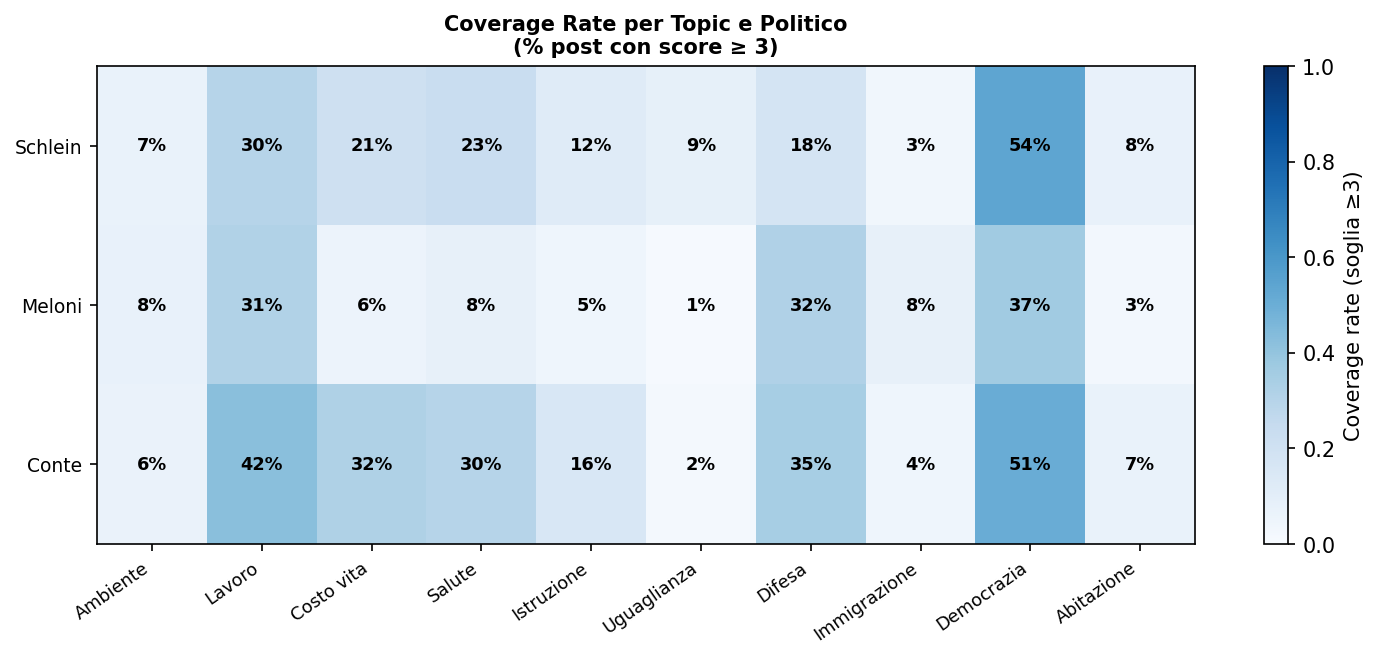
\includegraphics[width=0.92\textwidth]{coverage_heatmap.png}
\caption{Coverage Rate $c_i^{(p)}$ con $\tau=3$, dove le colonne sono
ordinate per priorit\`a giovanile decrescente, da rank $1$ a sinistra
fino a rank $10$ a destra, e le caselle pi\`u scure indicano i temi
pi\`u trattati dal politico. La rarefazione progressiva da destra
verso sinistra costituisce il nucleo del disallineamento, dato che i
temi pi\`u trattati dai politici sono quelli che i giovani indicano
come meno prioritari.}
\label{fig:cov}
\end{figure}

La heatmap della Figura~\ref{fig:cov} consente alcune letture
qualitative. La colonna a Coverage Rate pi\`u alto per Schlein e Conte
\`e \emph{democrazia e legalit\`a}, che fra i giovani occupa il rank
$8{,}5$, mentre per Meloni \emph{democrazia e legalit\`a} \`e in testa
a pari merito con \emph{difesa e sicurezza}, di rank giovanile $7$.
La colonna \emph{ambiente e clima}, prima per i giovani, \`e fra le
pi\`u chiare per tutti e tre i profili. Le colonne \emph{uguaglianza
di genere} e \emph{abitazione} risultano praticamente invisibili in
tutti e tre i profili, a fronte di una presenza moderata nella
survey, pari rispettivamente al $24\%$ e al $9\%$. I valori puntuali
con i relativi intervalli di confidenza sono riportati in
Tabella~\ref{tab:fullcov}.

\begin{table}[!htbp]
\centering
\caption{Coverage Rate in percentuale per tema e politico, con
$\tau=3$, accompagnati dall'intervallo di confidenza Wilson al $95\%$.
$N_{\text{Schlein}}=233$, $N_{\text{Meloni}}=278$,
$N_{\text{Conte}}=231$.}
\label{tab:fullcov}
\scriptsize
\begin{tabular}{l r r r}
\toprule
\textbf{Tema} & \textbf{Schlein \%\,[CI 95\%]} & \textbf{Meloni \%\,[CI 95\%]} & \textbf{Conte \%\,[CI 95\%]} \\
\midrule
Ambiente e clima        &  6.9\,[4.3--10.9]  &  7.6\,[5.0--11.3]  &  6.5\,[4.0--10.4] \\
Lavoro e economia       & 30.0\,[24.5--36.2] & 31.3\,[26.1--37.0] & 42.4\,[36.2--48.9] \\
Costo della vita        & 21.0\,[16.3--26.7] &  5.8\,[3.6--9.1]   & 32.0\,[26.4--38.3] \\
Salute e welfare        & 23.2\,[18.2--29.0] &  7.9\,[5.3--11.7]  & 29.9\,[24.3--36.1] \\
Istruzione e formazione & 12.0\,[8.5--16.8]  &  4.7\,[2.8--7.8]   & 15.6\,[11.5--20.8] \\
Uguaglianza di genere   &  8.6\,[5.6--12.9]  &  1.1\,[0.4--3.1]   &  1.7\,[0.7--4.4] \\
Difesa e sicurezza      & 17.6\,[13.2--23.0] & 32.0\,[26.8--37.7] & 34.6\,[28.8--41.0] \\
Immigrazione            &  3.4\,[1.8--6.6]   &  7.9\,[5.3--11.7]  &  4.3\,[2.4--7.8] \\
Democrazia e legalit\`a & 53.6\,[47.2--59.9] & 36.7\,[31.2--42.5] & 50.6\,[44.2--57.0] \\
Abitazione              &  7.7\,[4.9--11.9]  &  2.5\,[1.2--5.1]   &  6.9\,[4.3--11.0] \\
\bottomrule
\end{tabular}
\end{table}

\subsection{Sotto-rappresentazione di \emph{ambiente e clima}}

L'osservazione pi\`u marcata dello studio riguarda la posizione di
\emph{ambiente e clima} nelle quattro classifiche. Il tema occupa il
rank $1$ fra i giovani italiani da EP013EP, scivola al rank $9$ per
Schlein, al rank $8$ per Conte e al rank $6$ per Meloni a $\tau=3$.

Lo scarto \`e di otto posizioni di rank per Schlein, sette per Conte e
cinque per Meloni. Si tratta di un disallineamento strutturale che
attraversa lo spettro politico e non \`e dunque imputabile a un singolo
orientamento, dato che nessuno dei tre profili porta il tema sopra la
met\`a alta della propria classifica. Lo scarto sopravvive alla
perturbazione della soglia $\tau$ documentata in
Tabella~\ref{tab:tausens}, con la posizione di \emph{ambiente e
clima} che non sale mai al di sopra del rank $6$ in nessuno dei tre
profili e a nessuna delle tre soglie, e resta troppo ampio per
essere imputato al rumore di annotazione su un campione di oltre
$200$ post per profilo.

\subsection{Sovra-rappresentazione di \emph{democrazia e legalit\`a}}

Specularmente, il tema giovanilmente in posizione $8{,}5$ \`e in testa
alla classifica di tutti e tre i politici, con Coverage Rate osservati
del $54\%$ per Schlein, del $51\%$ per Conte e del $37\%$ per Meloni.
Il rank di vetta resta invariato per Schlein e per Meloni anche a
$\tau=2$ e $\tau=4$, e scivola al massimo al secondo posto per Conte
a $\tau=4$, segno che la posizione apicale non dipende dalla scelta
della soglia. La cornice politica del periodo, caratterizzata da
forti dinamiche di governo--opposizione, dossier giudiziari e
dibattito sul referendum sulla giustizia, fornisce una
spiegazione plausibile della centralit\`a del tema nelle agende dei
tre profili.

\subsection{Differenze di profilo}

I tre profili non sono fra loro equivalenti. Meloni \`e l'unico in cui
\emph{difesa/sicurezza} entra nei primi due rank, con Coverage del
$32\%$, coerentemente con l'agenda comunicativa di un governo in
carica, mentre \emph{immigrazione} \`e per Meloni al rank $4{,}5$ a
pari merito con \emph{salute/welfare} e per Schlein e Conte \`e in
fondo alla classifica. Schlein e Conte presentano classifiche simili,
dominate da \emph{democrazia/legalit\`a} e \emph{lavoro/economia}.
Le differenze osservate fra profili sono compatibili con i
posizionamenti politici documentati indipendentemente, e questa
coerenza interna offre un riscontro qualitativo della pipeline di
scoring, fermo restando il limite gi\`a discusso in \S 4.4--4.5,
ovvero che la validazione \`e su $30$ post per profilo e non
sull'ordinamento aggregato.

\section{Discussione}

I risultati sostengono la tesi di un disallineamento ampio e diffuso
fra le priorit\`a giovanili rilevate dall'Eurobarometro e l'agenda
comunicativa che i tre leader politici proiettano su Instagram. Il
caso pi\`u netto resta quello dell'ambiente, che si colloca
sistematicamente in fondo alle classifiche per tutti e tre i profili,
indipendentemente dall'orientamento politico.

\subsection{Fattore umano}

L'intera pipeline \`e automatizzata, ma in tre punti il giudizio umano
resta non sostituibile. Il primo \`e la scrittura del prompt di
scoring, ovvero la traduzione delle dieci categorie EB in istruzioni
operative per l'LLM, che costituisce un atto di interpretazione
semantica condizionante l'intera analisi. Il secondo \`e la
costruzione del campione di validazione e la sua annotazione, dato che
la qualit\`a dell'accordo inter-annotatore dipende dal modo in cui
sono stati selezionati i 30 post e dal modo in cui gli annotatori sono
stati istruiti. Il terzo \`e la lettura dei risultati, dato che le
metriche numeriche dicono che i ranking sono distanti, ma capire
perch\'e lo siano richiede competenze qualitative che non sono nei
dati e che riguardano la cornice politica, il formato della
piattaforma e l'agenda di governo.

\subsection{Limiti}\label{sec:limiti}

Il primo limite \`e la potenza statistica delle correlazioni globali
$\rho$ e $\tau_b$ con $n=10$ temi, dato che gli intervalli di
confidenza bootstrap di Tabella~\ref{tab:align} hanno larghezza di
ordine $0{,}3$ per tutti e tre i profili e l'intervallo di Meloni
include lo zero, condizione che impedisce di discriminare in modo
netto fra profili sulla base della sola correlazione globale. Il
secondo \`e la specificit\`a
del riferimento adottato. La pipeline \`e stata costruita per il confronto con la
popolazione giovanile italiana, ma lo stesso impianto metodologico si
presta ad altri segmenti sociali e ad altre survey, dato che
l'Eurobarometro non riflette al $100\%$ le priorit\`a giovanili in
ogni momento e che le priorit\`a stesse evolvono nel tempo. Una
replica con dati pi\`u recenti, con un riferimento diverso o su un
target diverso da quello giovanile potrebbe restituire ranking
parzialmente differenti.

\subsection{Disponibilit\`a di codice e dati}

Il codice sorgente della pipeline e gli artefatti dell'analisi, ovvero
CSV degli scoring, plot e ranking, sono pubblicati sul repository del
progetto all'indirizzo \url{https://github.com/Murkrow02/su.data}. I dati Eurobarometro sono
disponibili sul portale del Parlamento Europeo come Flash
Eurobarometer EP013EP~\cite{ep2024youth, ep2024youth_methodology}.

\bibliographystyle{ieeetr}
\bibliography{references}

\end{document}
